% 《物理实验报告模板.tex》的共同版式；所有实验模板均载入本文件。
\documentclass[UTF8,a4paper,10pt,fontset=fandol]{ctexart}
\usepackage[left=3.175cm,right=3.175cm,top=2.54cm,bottom=2.54cm]{geometry}
\usepackage{graphicx,tikz,pgfplots,needspace,adjustbox,booktabs,fancyhdr,lastpage,amsmath,amssymb,array,tabularx,longtable}
\pgfplotsset{compat=1.18}
\setlength{\parindent}{0pt}
\setlength{\parskip}{2pt}
\setlength{\headheight}{18pt}
\linespread{1}
\newcommand{\SetField}[2]{\expandafter\def\csname reportfield@#1\endcsname{#2}}
\makeatletter
\newcommand{\Field}[2][1.35cm]{%
  \ifcsname reportfield@#2\endcsname
    \expandafter\ifx\csname reportfield@#2\endcsname\@empty
      \underline{\makebox[#1]{\strut}}%
    \else\csname reportfield@#2\endcsname\fi
  \else\underline{\makebox[#1]{\strut}}\fi}
\makeatother
\newcommand{\MathField}[2][1.35cm]{%
  \ifcsname reportfield@math_#2\endcsname
    \csname reportfield@math_#2\endcsname
  \else\text{\Field[#1]{#2}}\fi}
\newcommand{\coverfield}[2]{%
  \noindent{\heiti\fontsize{18pt}{48pt}\selectfont
  \makebox[3.3cm][l]{#1}\underline{\makebox[8.8cm][c]{\Field[0pt]{#2}}}\par}}
\newcommand{\bindingline}[1][2.85]{%
  \begin{tikzpicture}[remember picture,overlay]
    \foreach \i in {0,...,38}{%
      \pgfmathsetmacro{\bindingy}{-#1-0.52*\i}%
      \ifnum\i=13\relax
        \node[inner sep=0pt] at ([xshift=1.05cm,yshift=\bindingy cm]current page.north west) {\songti\fontsize{10.5pt}{10.5pt}\selectfont 装};
      \else\ifnum\i=19\relax
        \node[inner sep=0pt] at ([xshift=1.05cm,yshift=\bindingy cm]current page.north west) {\songti\fontsize{10.5pt}{10.5pt}\selectfont 订};
      \else\ifnum\i=25\relax
        \node[inner sep=0pt] at ([xshift=1.05cm,yshift=\bindingy cm]current page.north west) {\songti\fontsize{10.5pt}{10.5pt}\selectfont 线};
      \else
        \pgfmathsetmacro{\bindingtop}{\bindingy+0.20}%
        \pgfmathsetmacro{\bindingbottom}{\bindingy-0.20}%
        \draw[line width=0.35pt,dash pattern=on 1.2pt off 1.8pt]
          ([xshift=1.05cm,yshift=\bindingtop cm]current page.north west)
          -- ([xshift=1.05cm,yshift=\bindingbottom cm]current page.north west);
      \fi\fi\fi}
  \end{tikzpicture}%
}
% 装订线印在每一页正文和原始数据页，续页也沿用母模板样式。
\newif\ifreportbinding
\AddToHook{shipout/foreground}{\ifreportbinding\bindingline\fi}
\fancypagestyle{report}{\fancyhf{}\fancyfoot[C]{第\thepage 页\quad 共\pageref{LastPage}页}\renewcommand{\headrulewidth}{0.4pt}}
\fancypagestyle{record}{\fancyhf{}\fancyhead[C]{原始数据记录单}\fancyfoot[C]{第\thepage 页\quad 共\pageref{LastPage}页}\renewcommand{\headrulewidth}{0.4pt}}
\newcommand{\ReportCover}[1]{%
  \thispagestyle{empty}\vspace*{1.0cm}
  \begin{center}
    
\includegraphics[width=8.184cm]{tongji_logo.jpeg}\par
    {\bfseries\fontsize{18pt}{24pt}\selectfont TONGJI UNIVERSITY\par}
    \vspace{1.5cm}{\heiti\fontsize{36pt}{44pt}\selectfont 物理实验报告\par}
  \end{center}
  \vspace{1.5cm}
  \coverfield{实验名称}{experiment}
  \coverfield{学生姓名}{student}
  \coverfield{学\hspace{1em}号}{student_id}
  \coverfield{组\hspace{1em}号}{group}
  \coverfield{实验日期}{date}
  \clearpage\reportbindingtrue\pagestyle{report}
  \begin{center}{\heiti\fontsize{14pt}{40pt}\selectfont #1\par}\end{center}}
\newcommand{\ReportSection}[1]{\Needspace{4\baselineskip}\par\vspace{0.35\baselineskip}{\heiti #1}\par}
\newcommand{\ReportSubsection}[1]{\Needspace{3\baselineskip}\par\vspace{0.2\baselineskip}{\bfseries #1}\par}
\newcommand{\ReportRecord}{%
  \clearpage\thispagestyle{record}
  \vspace*{0.6cm}（请将教师签字的实验数据记录单完整拍照粘贴至此处。）
}

% ===== 数据输入区开始 =====
\SetField{experiment}{用扭摆法测定物体转动惯量}
% 后端以 \SetField{字段名}{值} 填入数据；缺省值保持空白。
% 母模板封面字段：\Field{experiment} \Field{student} \Field{student_id} \Field{group} \Field{date}
% ===== 数据输入区结束 =====
\begin{document}\fontsize{10.5pt}{20pt}\selectfont
\ReportCover{用扭摆法测定物体转动惯量}
\ReportSection{实验目的}
1. 观察小角度扭摆，测量空盘与规则物体的周期并标定扭转常数。\par
2. 比较圆柱、圆筒、球和细杆的理论与实验转动惯量。\par
3. 改变两个对称滑块到转轴的距离，验证平行轴定理及惯量对距离平方的依赖。\par
\ReportSection{实验原理}
扭摆的回复力矩在小角度范围内近似满足 $M=-\kappa\theta$，运动方程为 $I\ddot\theta+\kappa\theta=0$，故
\[T=2\pi\sqrt{\frac I\kappa}.\]
以圆柱作标准物体，比较空盘周期 $T_0$ 和装圆柱周期 $T_1$，可由圆柱理论惯量 $I'_1=\frac{mD^2}{8}$ 求 $\kappa=\frac{4\pi^2I'_1}{T_1^2-T_0^2}$。其他物体的实验惯量由 $I_j=\frac{\kappa T_j^2}{4\pi^2}-I_0$ 求得。对两个质量均为 $m_s$ 的滑块，平行轴模型为 $I(x)=I_{\rm rod}+2I_s+2m_sx^2$。
以 $\Delta=T_1^2-T_0^2$ 记周期平方差。暂把标准圆柱的理论惯量视为已知常量，独立重复计时的传播公式为
\[u_\kappa=\kappa\sqrt{\left(\frac{2T_0u_{T_0}}{\Delta}\right)^2+
\left(\frac{2T_1u_{T_1}}{\Delta}\right)^2}.\]
\[\begin{aligned}
u_{I_0}^2={}&\left(\frac{2I'_1T_0T_1^2u_{T_0}}{\Delta^2}\right)^2+
\left(\frac{2I'_1T_1T_0^2u_{T_1}}{\Delta^2}\right)^2,\\
u_{I_j}^2={}&\left(\frac{2I'_1T_ju_{T_j}}{\Delta}\right)^2+
\left(\frac{2I'_1T_0(T_j^2-T_1^2)u_{T_0}}{\Delta^2}\right)^2\\
&+\left(\frac{2I'_1T_1(T_j^2-T_0^2)u_{T_1}}{\Delta^2}\right)^2\quad(j\ne1).
\end{aligned}\]
标定圆柱的 $I_1$ 与 $I'_1$ 由同一组周期构成，其计时项相消；完整不确定度还需计入圆柱质量、直径等仪器误差。
\begin{center}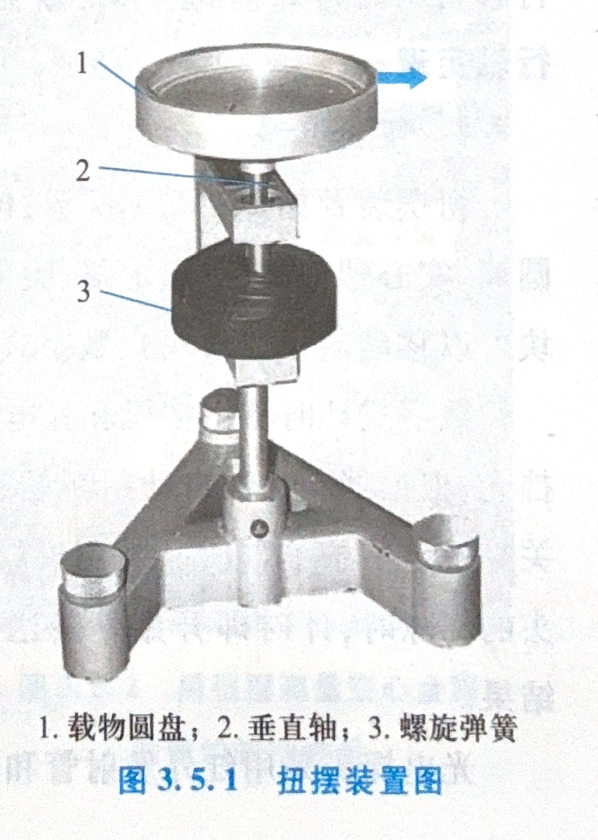
\includegraphics[width=3.4cm]{figures/torsion-apparatus.png}\par
{\small 扭摆装置示意图。}\end{center}
\ReportSection{实验内容}
\ReportSubsection{周期和几何量}
1. 调节底座水平与转轴竖直，保证载物盘空载时自由摆动；轻转一小角度后放手，避免向下压轴。\par
2. 测量空盘连续二十周期的总时长三次。依次安装圆柱、圆筒、木球和细杆，各计十周期并重复三次。\par
3. 测量各物体质量及必要的直径、长度；装置应居中、固定可靠，换物体时保持转轴条件一致。\par
\ReportSubsection{平行轴验证}
4. 把两个滑块关于转轴对称放在细杆上，量取滑块质心到轴的距离；在 5、10、15、20 cm 四个位置分别计五周期三次。\par
5. 将实验惯量与理论惯量对照，并以 $x^2$ 为横轴作图，检查线性关系。
\ReportSection{实验仪器}
扭摆实验仪、电子天平、游标卡尺、刻度尺和秒表。按计时周期数换算单周期，空盘、规则物体与滑块的周期数不同，不可混用。
\ReportSection{数据记录处理}
空盘计时为二十周期、其余物体计时为十周期的总时长（s），各重复三次：
\begin{center}\small\renewcommand{\arraystretch}{1.35}
\begin{tabular}{|c|c|c|c|c|c|}\hline
物体 & 计时周期数 & $t_1$/s & $t_2$/s & $t_3$/s & $\bar T$/s\\\hline
载物圆盘 & 20 & \Field[10mm]{time_disk_01} & \Field[10mm]{time_disk_02} & \Field[10mm]{time_disk_03} & \Field[10mm]{period_disk}\\\hline
实心圆柱 & 10 & \Field[10mm]{time_cylinder_01} & \Field[10mm]{time_cylinder_02} & \Field[10mm]{time_cylinder_03} & \Field[10mm]{period_cylinder}\\\hline
空心圆筒 & 10 & \Field[10mm]{time_tube_01} & \Field[10mm]{time_tube_02} & \Field[10mm]{time_tube_03} & \Field[10mm]{period_tube}\\\hline
木球 & 10 & \Field[10mm]{time_ball_01} & \Field[10mm]{time_ball_02} & \Field[10mm]{time_ball_03} & \Field[10mm]{period_ball}\\\hline
金属细杆 & 10 & \Field[10mm]{time_rod_01} & \Field[10mm]{time_rod_02} & \Field[10mm]{time_rod_03} & \Field[10mm]{period_rod}\\\hline
\end{tabular}
\end{center}
\noindent 单周期的计时标准不确定度 $u_{\bar T}$（空盘、圆柱、圆筒、木球、细杆依次为）
$\Field{period_disk_u}$、$\Field{period_cylinder_u}$、$\Field{period_tube_u}$、
$\Field{period_ball_u}$、$\Field{period_rod_u}$ s。
\noindent 几何量：圆柱 $m_1=\Field{mass_cylinder_g}$ g、$D_1=\Field{diameter_cylinder_mm}$ mm；
圆筒 $m_2=\Field{mass_tube_g}$ g、$D_o=\Field{diameter_tube_outer_mm}$ mm、$D_i=\Field{diameter_tube_inner_mm}$ mm；
木球 $m_3=\Field{mass_ball_g}$ g、$D_3=\Field{diameter_ball_mm}$ mm；
细杆 $m_4=\Field{mass_rod_g}$ g、$l_4=\Field{length_rod_mm}$ mm。
\[\kappa=(\MathField{torsion_constant}\pm\MathField{torsion_constant_u})\,\mathrm{N\,m}.\]
\[I_0=(\MathField{empty_inertia}\pm\MathField{empty_inertia_u})\,\mathrm{kg\,m^2}.\]
\begin{center}\small\renewcommand{\arraystretch}{1.35}
\begin{tabular}{|c|c|c|c|c|}\hline
物体 & $I_{
m th}$/kg m$^2$ & $I_{
m exp}$/kg m$^2$ & $u_I$/kg m$^2$ & 百分差/\%\\\hline
实心圆柱 & $\MathField{theory_cylinder}$ & $\MathField{experiment_cylinder}$ & $\MathField{experiment_cylinder_u}$ & \Field[10mm]{error_cylinder}\\\hline
空心圆筒 & $\MathField{theory_tube}$ & $\MathField{experiment_tube}$ & $\MathField{experiment_tube_u}$ & \Field[10mm]{error_tube}\\\hline
木球 & $\MathField{theory_ball}$ & $\MathField{experiment_ball}$ & $\MathField{experiment_ball_u}$ & \Field[10mm]{error_ball}\\\hline
金属细杆 & $\MathField{theory_rod}$ & $\MathField{experiment_rod}$ & $\MathField{experiment_rod_u}$ & \Field[10mm]{error_rod}\\\hline
\end{tabular}
\end{center}
\noindent 表中 $u_I$ 仅由重复计时传播；标定圆柱的计时贡献与其标准惯量相消，几何量和质量的仪器不确定度未计入。
\ReportSection{平行轴定理验证}
\noindent 单滑块质量 $m_s=\Field{slider_mass_g}$ g；单滑块自身惯量 $I_s=\Field{slider_self_inertia}$ kg m$^2$。
\noindent 滑块计时为五周期的总时长（s），各重复三次。
\begin{center}\small\renewcommand{\arraystretch}{1.35}
\begin{tabular}{|c|c|c|c|c|c|c|}\hline
$x$/cm & $t_1$/s & $t_2$/s & $t_3$/s & $\bar T$/s & $I_{\rm th}$ & $I_{\rm exp}$\\\hline
5 & \Field[10mm]{slider_time_5_01} & \Field[10mm]{slider_time_5_02} & \Field[10mm]{slider_time_5_03} & \Field[10mm]{slider_period_5} & $\MathField{slider_theory_5}$ & $\MathField{slider_experiment_5}$\\\hline
10 & \Field[10mm]{slider_time_10_01} & \Field[10mm]{slider_time_10_02} & \Field[10mm]{slider_time_10_03} & \Field[10mm]{slider_period_10} & $\MathField{slider_theory_10}$ & $\MathField{slider_experiment_10}$\\\hline
15 & \Field[10mm]{slider_time_15_01} & \Field[10mm]{slider_time_15_02} & \Field[10mm]{slider_time_15_03} & \Field[10mm]{slider_period_15} & $\MathField{slider_theory_15}$ & $\MathField{slider_experiment_15}$\\\hline
20 & \Field[10mm]{slider_time_20_01} & \Field[10mm]{slider_time_20_02} & \Field[10mm]{slider_time_20_03} & \Field[10mm]{slider_period_20} & $\MathField{slider_theory_20}$ & $\MathField{slider_experiment_20}$\\\hline
\end{tabular}
\end{center}
\noindent 滑块单周期的计时标准不确定度（按 $x=5,10,15,20$ cm 顺序）：
$\Field{slider_period_5_u}$、$\Field{slider_period_10_u}$、
$\Field{slider_period_15_u}$、$\Field{slider_period_20_u}$ s。
\noindent 滑块实验惯量的计时标准不确定度（按 $x=5,10,15,20$ cm 顺序）：
$\Field{slider_experiment_5_u}$、$\Field{slider_experiment_10_u}$、
$\Field{slider_experiment_15_u}$、$\Field{slider_experiment_20_u}$ kg m$^2$。
\noindent 理论模型 $I_{\rm th}(x)=I'_{\rm rod}+2I_s+2m_sx^2$；
滑块的位移应按其质心到转轴的距离计。

\ReportSection{平行轴定理的数据图}
横轴取滑块距离平方 $x^2$（cm$^2$），纵轴取总惯量的 $10^{-3}\,\mathrm{kg\,m^2}$ 数值。散点是周期换算的实验结果，直线连接对应理论值；两条序列均来自本次读数和输入的滑块质量。
\begin{center}\begin{tikzpicture}
\begin{axis}[width=.82\textwidth,height=4.8cm,xlabel={$\frac{x^2}{\mathrm{cm^2}}$},ylabel={$\frac{I}{10^{-3}\,\mathrm{kg\,m^2}}$},grid=both,legend pos=north west]
\addplot+[only marks,mark=*,mark size=2pt] coordinates {\PlotCoordinates{slider_graph_points}};
\addlegendentry{实测惯量}
\addplot+[no marks,thick,blue] coordinates {\PlotCoordinates{slider_graph_theory_points}};
\addlegendentry{平行轴理论}
\end{axis}\end{tikzpicture}\end{center}
\ReportSection{讨论与分析}
\ReportSubsection{图形与模型}
若平行轴定理适用，$I$ 对 $x^2$ 的点应近似落在直线上，斜率由两个滑块的质量决定。若图中随位置出现系统偏离，应检查距离是否从滑块质心量起、两个滑块是否对称，以及滑块本身惯量是否计入。\par
\ReportSubsection{主要误差}
计时起止点不一致、转轴摩擦、振幅过大和物体偏心都会改变周期。圆柱用于标定 $\kappa$，其质量和直径误差会传递到所有实验惯量。比较理论值时必须扣除空盘惯量 $I_0$。\par
\ReportSubsection{思考题}
为何空盘计时二十周期，而物体只计十周期？空盘周期较短，扩大总计时长度可以减小启停反应时间的相对影响。为何使用两个对称滑块？对称布置可以减少质心偏离转轴引起的附加晃动。
\ReportSection{实验结论}
由圆柱与空盘的周期差标定扭转常数 $\kappa=(\MathField{torsion_constant}\pm\MathField{torsion_constant_u})\,\mathrm{N\,m}$，再求其他物体惯量。这里的不确定度只计重复计时的贡献。滑块位置变化所得散点应与 $I=I_{\rm rod}+2I_s+2m_sx^2$ 的平方关系比较，不能只凭周期随距离变大作结论。

\ReportRecord
% ===== 原始数据图片插入区 =====
\end{document}
